\clearpage
\section{Auswertung}
\label{sec:auswertung}

	\subsection{Klemmspannungskurven}
	\label{subsec:kurven}
		Zun"achst wird f"ur jede Spannungsquelle eine lineare Ausgleichsrechnung mit Hilfe von \emph{phython} f"ur die Funktion \eqref{uk} durchgef"uhrt.
		Der y-Achsenabschnitt entpricht dabei der Leerlaufspannung $U_0$ und die Steigung dem Innenwiderstand $R_\mathrm{i}$ der jeweiligen Spannungsquelle.
		Abbildungen \ref{fig:graph_monozelle} bis \ref{fig:graph_sinus} zeigen die Graphen, Tabelle \ref{table:monozelle} beinhaltet die Messwerte.
		Die Ungenauigkeit der Messger"ate liegt bei

		\begin{eqnarray*}
			\Delta I & = & \pm \SI{1.5}{\percent} \,, \\
			\Delta U & = & \pm \SI{2}{\percent} \,.
		\end{eqnarray*}

		Zudem gilt f"ur die Leistung $P$:

		\begin{eqnarray*}
			P & = & UI \,, \\
			\Delta P & = & \sqrt{(I \Delta U)^2 + (U \Delta I)^2} \,. 
		\end{eqnarray*}

		\begin{table}[h!]
			\begin{center}
				\caption{Strom- und Spannungswerte der verschiedenen Spannungsquellen bei variierten Lastwiderst"anden $R_\mathrm{a}$. \label{table:monozelle}}
				\begin{tabular}{|c|c|r||c|c|r||c|c|r|}
					\hline
						\multicolumn{3}{|c||}{Monozelle} & \multicolumn{3}{c||}{Rechteckspannung} & \multicolumn{3}{c|}{Sinusspannung} \\
					\hline
						$I [\SI{}{\milli \ampere}]$ & $U_\mathrm{k} [\SI{}{\volt}]$ & $P [\SI{}{\milli \watt}]$ &
						$I [\SI{}{\milli \ampere}]$ & $U_\mathrm{k} [\SI{}{\milli \volt}]$ & $P [\SI{}{\micro \watt}]$ &
						$I [\SI{}{\milli \ampere}]$ & $U_\mathrm{k} [\SI{}{\volt}]$ & $P [\SI{}{\micro \watt}]$\\
					\hline 
					\hline
						84	&	$\SI{.083}{}$ & $\SI{06.97 (17)}{}$ & $\SI{7.7}{}$ & 40 & $\SI{308 (8)}{}$ & $\SI{1.80}{}$ & $\SI{0.09}{}$ & $\SI{162 (4)}{}$ \\
76	&	$\SI{.240}{}$ & $\SI{18.24 (46)}{}$ & $\SI{6.5}{}$ & 50 & $\SI{325 (8)}{}$ & $\SI{1.50}{}$ & $\SI{0.12}{}$ & $\SI{180 (4)}{}$ \\
66	&	$\SI{.280}{}$ & $\SI{18.48 (46)}{}$ & $\SI{5.1}{}$ & 65 & $\SI{332 (8)}{}$ & $\SI{1.00}{}$ & $\SI{0.17}{}$ & $\SI{170 (4)}{}$ \\
58	&	$\SI{.570}{}$ & $\SI{33.06 (83)}{}$ & $\SI{4.2}{}$ & 70 & $\SI{294 (7)}{}$ & $\SI{0.70}{}$ & $\SI{0.20}{}$ & $\SI{140 (4)}{}$ \\
54	&	$\SI{.640}{}$ & $\SI{34.56 (86)}{}$ & $\SI{3.5}{}$ & 75 & $\SI{263 (7)}{}$ & $\SI{0.60}{}$ & $\SI{0.22}{}$ & $\SI{132 (3)}{}$ \\
47	&	$\SI{.750}{}$ & $\SI{35.25 (88)}{}$ & $\SI{3.1}{}$ & 80 & $\SI{248 (6)}{}$ & $\SI{0.55}{}$ & $\SI{0.23}{}$ & $\SI{127 (3)}{}$ \\
43	&	$\SI{.770}{}$ & $\SI{33.11 (83)}{}$ & $\SI{2.7}{}$ & 85 & $\SI{230 (6)}{}$ & $\SI{0.45}{}$ & $\SI{0.24}{}$ & $\SI{108 (3)}{}$ \\
41	&	$\SI{.780}{}$ & $\SI{31.98 (80)}{}$ & $\SI{2.3}{}$ & 85 & $\SI{196 (5)}{}$ & $\SI{0.38}{}$ & $\SI{0.24}{}$ & $\SI{091 (2)}{}$ \\
38	&	$\SI{.810}{}$ & $\SI{30.78 (77)}{}$ & $\SI{2.0}{}$ & 90 & $\SI{180 (4)}{}$ & $\SI{0.32}{}$ & $\SI{0.25}{}$ & $\SI{080 (2)}{}$ \\
36	&	$\SI{.820}{}$ & $\SI{29.52 (74)}{}$ & $\SI{1.8}{}$ & 90 & $\SI{162 (4)}{}$ & $\SI{0.27}{}$ & $\SI{0.25}{}$ & $\SI{068 (2)}{}$ \\
34	&	$\SI{.820}{}$ & $\SI{27.88 (70)}{}$ & $\SI{1.7}{}$ & 90 & $\SI{153 (4)}{}$ & $\SI{0.25}{}$ & $\SI{0.25}{}$ & $\SI{062 (2)}{}$ \\
					\hline 
				\end{tabular}
			\end{center}
		\end{table}

		\begin{figure}[h]
			\centering
			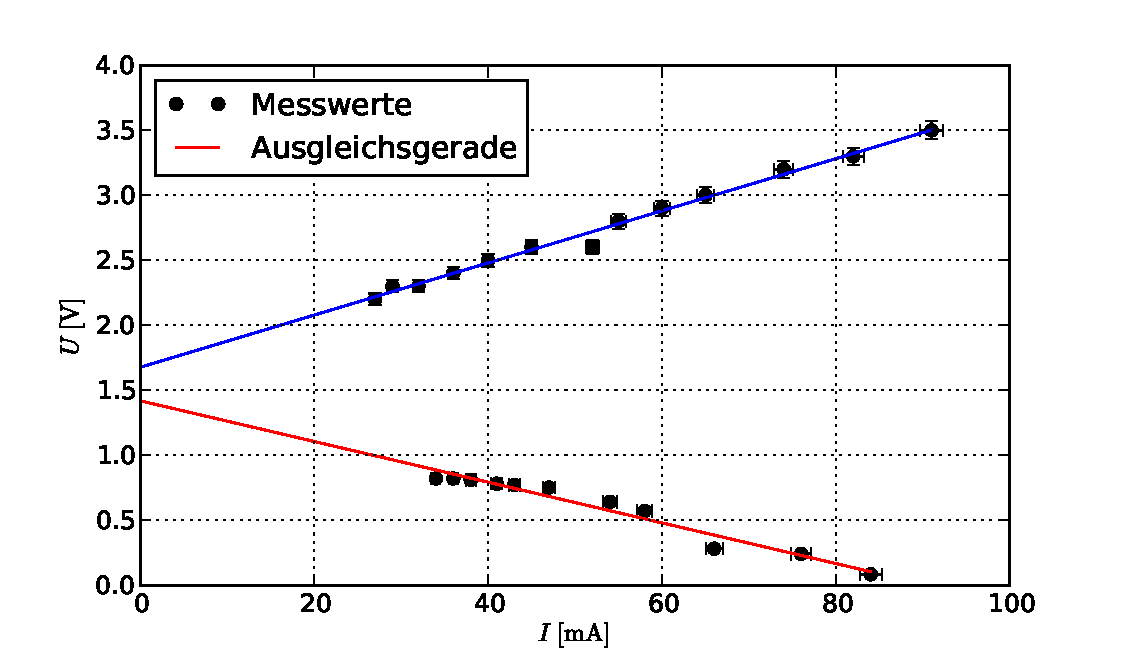
\includegraphics[width = 15cm]{img/graph_monozelle.pdf}
			\caption{Spannungs- Stromkurve der Monozelle. \label{fig:graph_monozelle}}
		\end{figure}

		\begin{figure}[h]
			\centering
			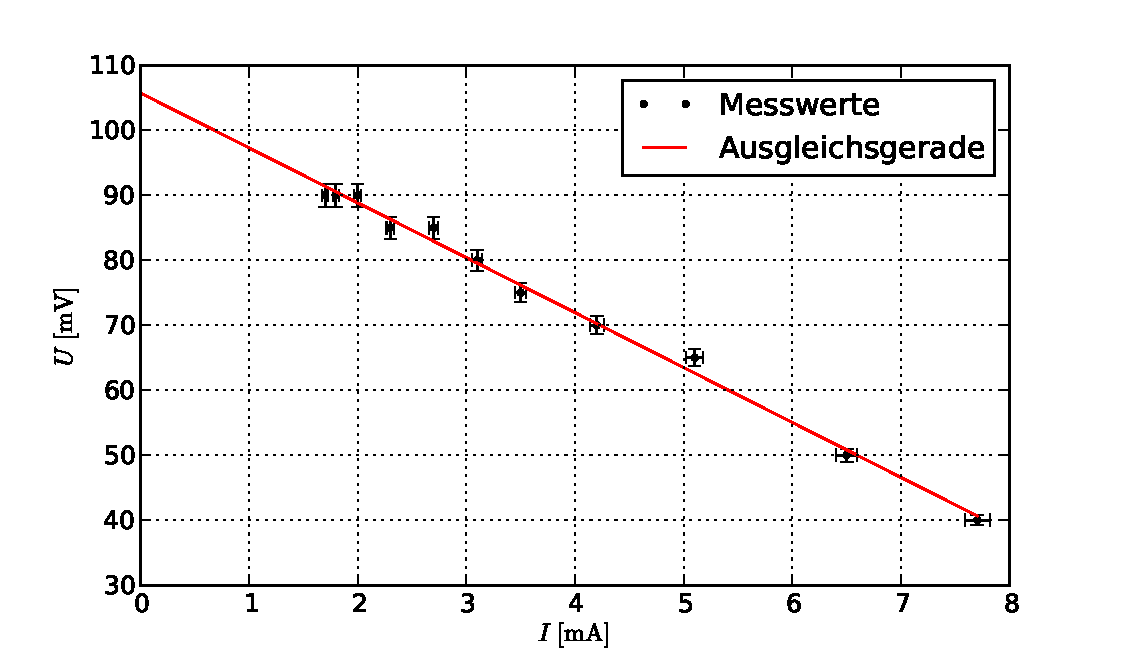
\includegraphics[width = 15cm]{img/graph_rechteck.pdf}
			\caption{Spannungs- Stromkurve der Rechteckspannung \label{fig:graph_rechteck}}
		\end{figure}

		\begin{figure}[h]
			\centering
			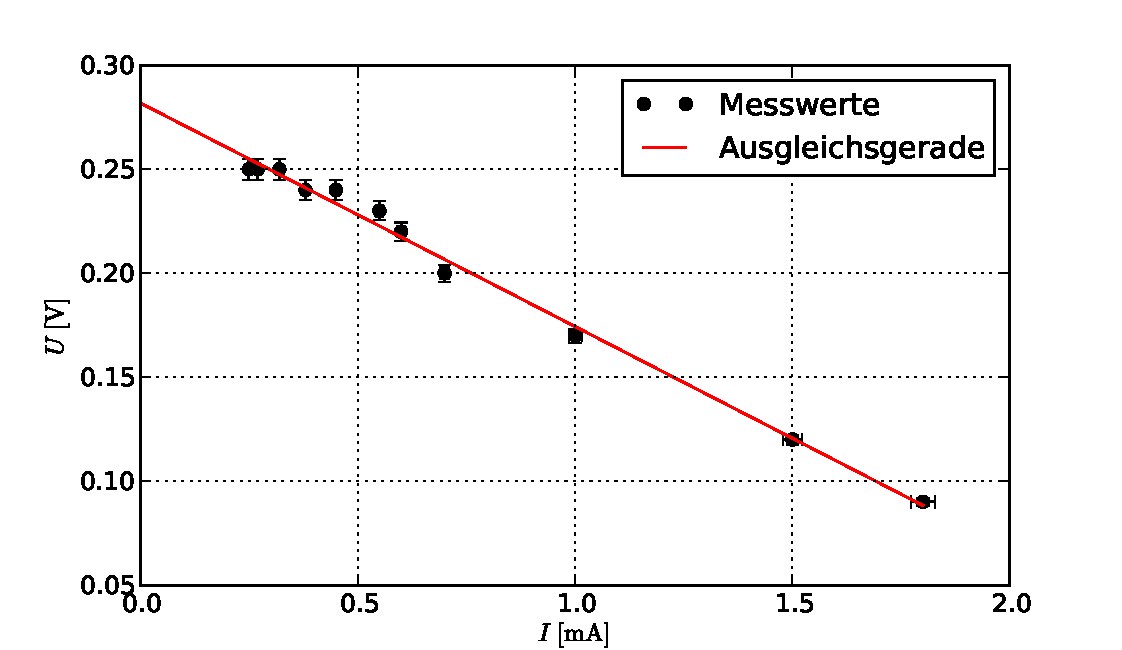
\includegraphics[width = 15cm]{img/graph_sinus.pdf}
			\caption{Spannungs- Stromkurve der Sinusspannung \label{fig:graph_sinus}}
		\end{figure}

	\clearpage

	\subsection{Innenwiderstand $R_\mathrm{i}$ und Leerlaufspannung $U_0$}
	\label{subsec:ri-u0}
		Die Ausgleichsrechnung in Kapitel \ref{subsec:kurven} liefert die Werte f"ur die jeweiligen Innenwiderst"ande $R_\mathrm{i}$ und Leerlaufspannungen $U_0$ der verschiedenen Spannungsquellen.
		Tabelle \ref{table:ri-u0} beinhaltet die Werte.

		\begin{table}[h!]
			\begin{center}
				\caption{Innenwiderstand $R_\mathrm{i}$ und Leerlaufspannung $U_0$. \label{table:ri-u0}}
				\begin{tabular}{|r|r|c|}
					\hline
						Spannungsquelle & \multicolumn{1}{|c|}{$R_\mathrm{i} [\SI{}{\ohm}]$} & $U_0 [\SI{}{\volt}]$ \\ 
					\hline 
					\hline
						Monozelle & $\SI{15.7 (11)}{}$ & $\SI{1.418 (60)}{}$ \\
						Monozelle, Gegenspannung & $\SI{20.1 (6)}{}$ & $\SI{1.676 (34)}{}$ \\
						Rechteckspannung & $\SI{107.6 (30)}{}$ & $\SI{.106 (1)}{}$ \\
						Sinusspannung & $\SI{8.5 (2)}{}$ & $\SI{.282 (3)}{}$ \\ 
					\hline 
				\end{tabular}
			\end{center}
		\end{table}

	\subsection{Systematische Fehler}
	\label{subsec:fehler}
		Der Systematische Fehler $\Delta_\mathrm{s} U_0$ bei der direkten Messung der Leerlaufspannung betr"agt nach Umstellen von Gleichung \eqref{uk}:

		\begin{equation*}
			\Delta_\mathrm{s} U_0 = U_\mathrm{k} \frac{R_\mathrm{i}}{R_\mathrm{a}} \,.
		\end{equation*}

		Mit einem Au"senwiderstand im Voltmeter von $R_\mathrm{a} \approx \SI{10}{\mega \ohm}$ und der direkt gemessenen Spannung

		\begin{equation*}
			U_0 = \SI{1.65}{\volt} \,,
		\end{equation*}
		
		folgt der Fehler

		\begin{equation*}
			\Delta_\mathrm{s} U_0 = \SI{2.59}{\micro \ohm} \,.
		\end{equation*}

		Das entspricht einem relativen Fehler $\delta_\mathrm{s}$ von $\delta_\mathrm{s} = \SI{1.57e-4}{\percent}$.

		Schlie"st man das Voltmeter nicht wie vorgegeben an, sondern hinter dem Amperemeter, f"allt in diesem -- zus"atzlich zur Leerlaufspannung $U_0$ -- eine Spannung $U_\mathrm{A}$ ab.

	\subsection{Leistungsdiagramm}
	\label{subsec:leistung}
		Im folgenden Diagramm \ref{fig:graph_monozelle_leistung} ist die Leistung $P$, die im Belastungswiderstand $R_\mathrm{a}$ umgesetzt wird, aufgetragen.
		Zus"atzlich ist der Graph der theoretisch errechneten Leistungskurve $N = f(R_\mathrm{a})$ eingetragen.
		Die Leistungskurve berechnet sich mit Gleichung \eqref{eqn:leistung} nach

		% \begin{equation*}
		% 	N = I^2 R_\mathrm{a} = \frac{{U_0}^2 R_\mathrm{a}}{\left(R_\mathrm{i} + R_\mathrm{a}\right)^2} \,.
		% \end{equation*}

		Hierbei werden die Werte des Innenwiderstandes $R_\mathrm{i}$ und der Leerlaufspannung $U_0$ ohne Gegenspannung aus Kapitel \ref{subsec:ri-u0} verwendet.

		\begin{figure}[h]
			\centering
			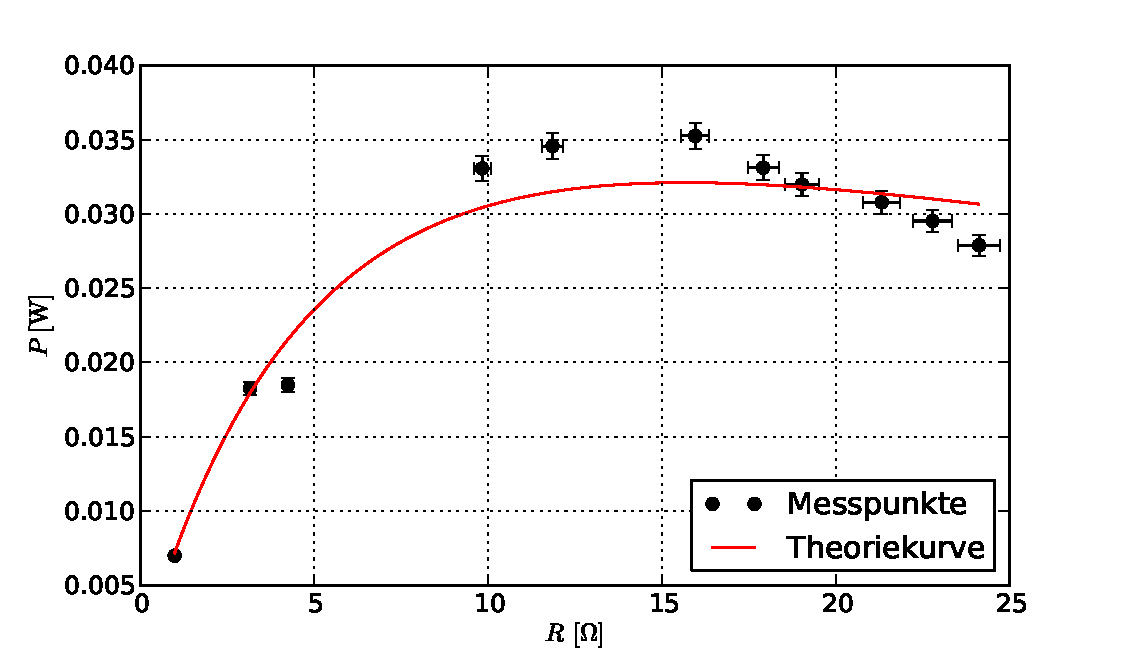
\includegraphics[width = 15cm]{img/graph_monozelle_leistung.pdf}
			\caption{Leistungsdiagramm der Monozelle mit theoretischer Leistungskurve. \label{fig:graph_monozelle_leistung}}
		\end{figure}